%\documentstyle[epsf,twocolumn]{jarticle}       %LaTeX2e仕様
%\documentclass[twocolumn]{jarticle}     %pLaTeX2e仕様(platex.exeの場合)
\documentclass[onecolumn]{ujarticle}   %pLaTeX2e仕様(uplatex.exeの場合)
%%%%%%%%%%%%%%%%%%%%%%%%%%%%%%%%%%%%%%%%%%%%%%%%%%%%%%%%%%%%%%
%%
%%  基本バージョン
%%
%%%%%%%%%%%%%%%%%%%%%%%%%%%%%%%%%%%%%%%%%%%%%%%%%%%%%%%%%%%%%%%%
\setlength{\topmargin}{-45pt}
%\setlength{\oddsidemargin}{0cm}
\setlength{\oddsidemargin}{-7.5mm}
%\setlength{\evensidemargin}{0cm}
\setlength{\textheight}{24.1cm}
%setlength{\textheight}{25cm}
\setlength{\textwidth}{17.4cm}
%\setlength{\textwidth}{172mm}
\setlength{\columnsep}{11mm}

%\kanjiskip=.07zw plus.5pt minus.5pt


% 【節が変わるごとに (1.1)(1.2) … (2.1)(2.2) と数式番号をつけるとき】
%\makeatletter
%\renewcommand{\theequation}{%
%\thesection.\arabic{equation}} %\@addtoreset{equation}{section}
%\makeatother

%\renewcommand{\arraystretch}{0.95} 行間の設定
%%%%%%%%%%%%%%%%%%%%%%%%%%%%%%%%%%%%%%%%%%%%%%%%%%%%%%%%
%\usepackage{graphicx}   %pLaTeX2e仕様(\documentstyle ->\documentclass)
\usepackage[dvipdfmx]{graphicx}
\usepackage{subcaption}
\usepackage{multirow}
\usepackage{amsmath}
\usepackage{url}
\usepackage{ulem}
%%%%%%%%%%%%%%%%%%%%%%%%%%%%%%%%%%%%%%%%%%%%%%%%%%%%%%%%
\begin{document}

	%bibtex用の設定
	%\bibliographystyle{ujarticle}
	% \twocolumn[
	\noindent

	\hspace{1em}
	2020 年 02 月 07 日
	ゼミ資料
	\hfill
	M1 寺内 光

	\vspace{2mm}

	\hrule

	\begin{center}
		{\Large \bf 進捗報告}
	\end{center}


	\hrule
	\vspace{3mm}
	% ]

	% ‚ここから 文章 Start!
	\section{今週やったこと}
	\begin{itemize}{
		\item{台詞が空のものをデータセットから除くデータ整形}
		\item{分散表現間の距離の指標をいくつか試した}
		\item{L1Lossを用いて学習}
		\item{バッチをインデックスと紐付け,画像に対応する台詞の予測結果を取得}
	}
	\end{itemize}

	\subsection{台詞が空のものをデータセットから除くデータ整形}
	台詞が空のものが候補に複数入る可能性があり,MRR が不当に上がる可能性があるので削除.また,規定のバッチサイズに満たないバッチを MRR の計算に使わないように変更した.

	\subsection{分散表現間の距離の指標をいくつか試した}
	学習語,予測された分散表現のマッチングを取る際の距離の指標として,ユークリッド距離を用いていたが,その距離の指標を試験的に色々変えてみた.損失関数を MSE として それぞれ30 エポック実験を回した.
	表 \ref{tab:result} に結果を示す.

	\begin{table}[h]
		\vspace{-3mm}
		\centering
		\caption{画像→台詞マッチング識別結果(MRR)}
		\label{tab:result}
		\begin{tabular}{|c|c|c|c|c|} \hline
			用いた距離指標&訓練識別率&評価識別率&テスト識別率&ベースライン\\ \hline\hline
			euclidean&0.668&0.358&0.222&0.293\\ \hline
			cosine&0.704&0.338&0.248&0.293\\ \hline
			canberra&0.524&0.318&0.260&0.293\\ \hline
			chebyshev&0.292&0.293&0.256&0.293\\ \hline
			cityblock&0.580&0.332&0.262&0.293\\ \hline
			correlation&0.677&0.384&0.227&0.293\\ \hline
			minkowski&0.714&0.357&0.248&0.293\\ \hline
			sqeuclidean&0.640&0.337&0.236&0.293\\ \hline
		\end{tabular}
	\end{table}

	どの距離指標も現時点ではあまり大差ないことが分かった(そもそも学習ができてないので).

	\subsection{L1Lossを用いて学習}
	損失関数の方を変えて学習を回したが,やはり改善は見られずという感じ.

	\subsection{バッチをインデックスと紐付け,画像に対応する台詞の予測結果を取得}
	予測結果に最もマッチングする台詞をとってこれるように改良し,損失関数に MSE, 距離の指標にユークリッド距離を使った時にどのようなマッチング結果が得られたか取得した.
	下に valid データに対する結果および test データに対する結果を示す.

	\begin{table}[h]
		\vspace{-3mm}
		\centering
		\caption{画像→台詞マッチング結果(valid)}
		\label{tab:result}
		\begin{tabular}{|c|p{11cm}|} \hline
			用いた画像&台詞(距離)\\ \hline\hline
			\multirow{1}{*}{YouchienBoueigumi-332.jpg}&あ あの 小 娘 め ・ ・ まさか 新井 先生 の 事 を ・・・ ・ よかった じゃ ない か ライバル が 出現 して(20.166) \\ \cline{2-2}
			&だって あんまり 遊び に 行か ない し ハデ な 服 も 買わ ない し ひと 月 いくら くらい 遣って んです か ?(20.410) \\ \cline{2-2}
			&いや … その 注目 さ れる と … ほら … え(20.582)\\ \hline
			\multirow{1}{*}{KoukouNoHitotachi-876.jpg}&これ は この前 着て った し これ は 貧乏 くさい し ああ あ 着て いく 服 が ない ! どー し よー(20.569) \\ \cline{2-2}
			&着 なく なった 服 は 近所 の 健一 くん って 子 に あげる んだ ボランティア 部 部長 貧乏で 服 が 買え ない らしくて ね 小学生 だ けど 体 が 大きい から ボク の でも サイズ が あう んだ(20.651) \\ \cline{2-2}
			&ああいう の も 悪く ない なあ それ ・ ・ ・ やばい よ 絶対 ・ ・ ・(21.184) \\ \hline
		\end{tabular}
	\end{table}

	\begin{figure}[h]
		\centering
		\begin{subfigure}{0.49\columnwidth}
			\centering
			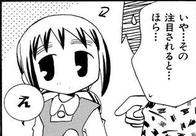
\includegraphics[width=0.9\columnwidth]{data/YouchienBoueigumi-332.jpg}
				\caption{YouchienBoueigumi-332.jpg}
		\end{subfigure}
		\begin{subfigure}{0.49\columnwidth}
			\centering
			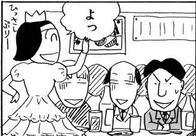
\includegraphics[width=0.9\columnwidth]{data/KoukouNoHitotachi-876.jpg}
				\caption{KoukouNoHitotachi-876.jpg}
		\end{subfigure}
		\caption{valid 用いた画像}
		\label{fig:target}
	\end{figure}

	\begin{table}[h]
		\vspace{-3mm}
		\centering
		\caption{画像→台詞マッチング結果(test)}
		\label{tab:result}
		\begin{tabular}{|c|p{11cm}|} \hline
			用いた画像&台詞(距離)\\ \hline\hline
			\multirow{1}{*}{shonen-054.jpg}&手作り な んです か ? ほとんど 冷凍 食品 詰めた だけ よ …(23.256) \\ \cline{2-2}
			&国際 会議 で スペイン に いる B さん から だ (23.590) \\ \cline{2-2}
			&じゃあ チョコ です ね チョコ は 一 つ しか ない し 、 悪い よ〜 別に 気 に し ませ ん が …(23.691) \\ \hline
			\multirow{1}{*}{shonen-064.jpg}&絶対 ドン 引き する と 思った のに なあ アイドル と か 好きな んだ〜(20.080) \\ \cline{2-2}
			&この 服 可愛い ね え!?(20.445) \\ \cline{2-2}
			&恥ずかしい …(21.047) \\ \hline
		\end{tabular}
	\end{table}

	\begin{figure}[h]
		\centering
		\begin{subfigure}{0.49\columnwidth}
			\centering
			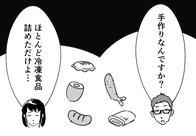
\includegraphics[width=0.9\columnwidth]{data/shonen-054.jpg}
				\caption{shonen-054.jpg}
		\end{subfigure}
		\begin{subfigure}{0.49\columnwidth}
			\centering
			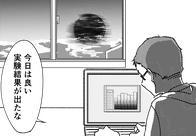
\includegraphics[width=0.9\columnwidth]{data/shonen-064.jpg}
				\caption{shonen-064.jpg}
		\end{subfigure}
		\caption{test 用いた画像}
		\label{fig:target}
	\end{figure}


	\section{来週の予定}\noindent
	台詞間にデリミタを入れた実験を試す(unknown トークンとして扱われるだけなので本質的に影響はなさそうな気も..?)

	また,画像と台詞の分散表現を 2 次元プロットした解析もしたい.
	%
	% \bibliographystyle{unsrt}
	% \bibliography{2020_01_10_terauchi}

\end{document}
